\chapter{Data Analysis}\label{chap:dataanlysis}
This project will investigate if there exists a cointegrating relation between the four cryptocurrencies namely, Bitcoin, Ethereum, Solana and Ripple. In this chapter a short introduction to data will be made and afterwards the data will be examined. This will be done with the use of visual interpretation of plots aswell as quantitativ tests.

\section{Data Introduction}
The data that has been used can be found at yahoo  [ref].\\
The data which has been chosen for this project, consists of opening prices, the daily lowest prices, the daily highest price and the closing prices all in USD. The chosen period is from 10th of December 2020 to 10th October 2024. These four has been chosen on the basis, they are the largest coins measured on market capitalization, and the fact that none of them are so called stable coins, which is a coin pegged to a FIAT currency. The data from these Crypto currency's have been cleaned to only contain closing prices. It has then been check for NA values, of which there are none present. The data is then split into two parts a training data set, which consist of the first $90\%$ of the data, and a validation data set, which consist of the last $10\%$. The training set is used for fitting different models. Furthermore model validation will be performed upon this data set. The validation set has been used to investigate the forecasting ability and accuracy of the models.\\
We will now precede with checking the training data
\section{Leveled graph}
The four crypto currencies' closing prices in levels have been plotted below.
\begin{figure}[H]
  \centering
  \subfloat[][Bitcoin]{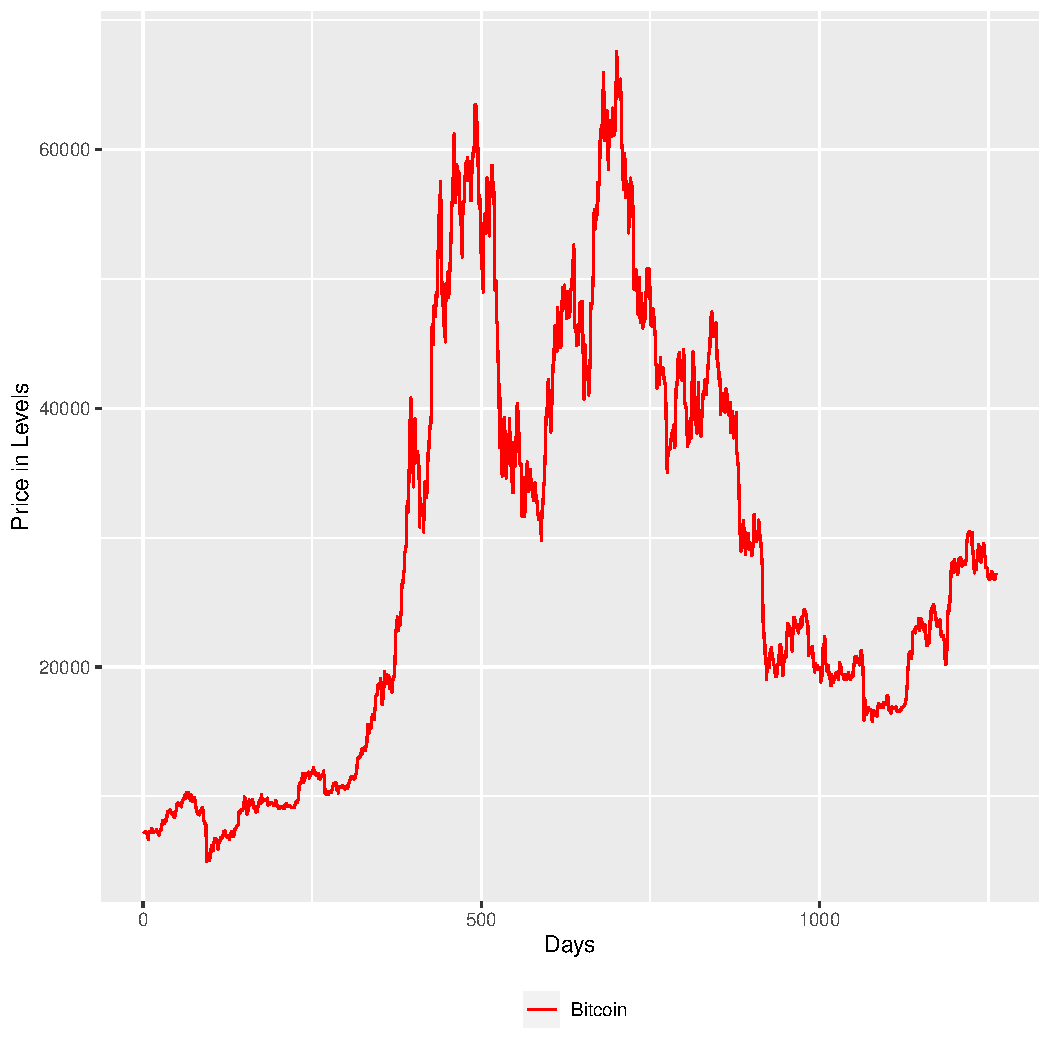
\includegraphics[width=.4\textwidth]{1.Projekt_kode/Billeder/Crypto_in_levels_Bitcoin.pdf}}\quad
  \subfloat[][Ethereum]{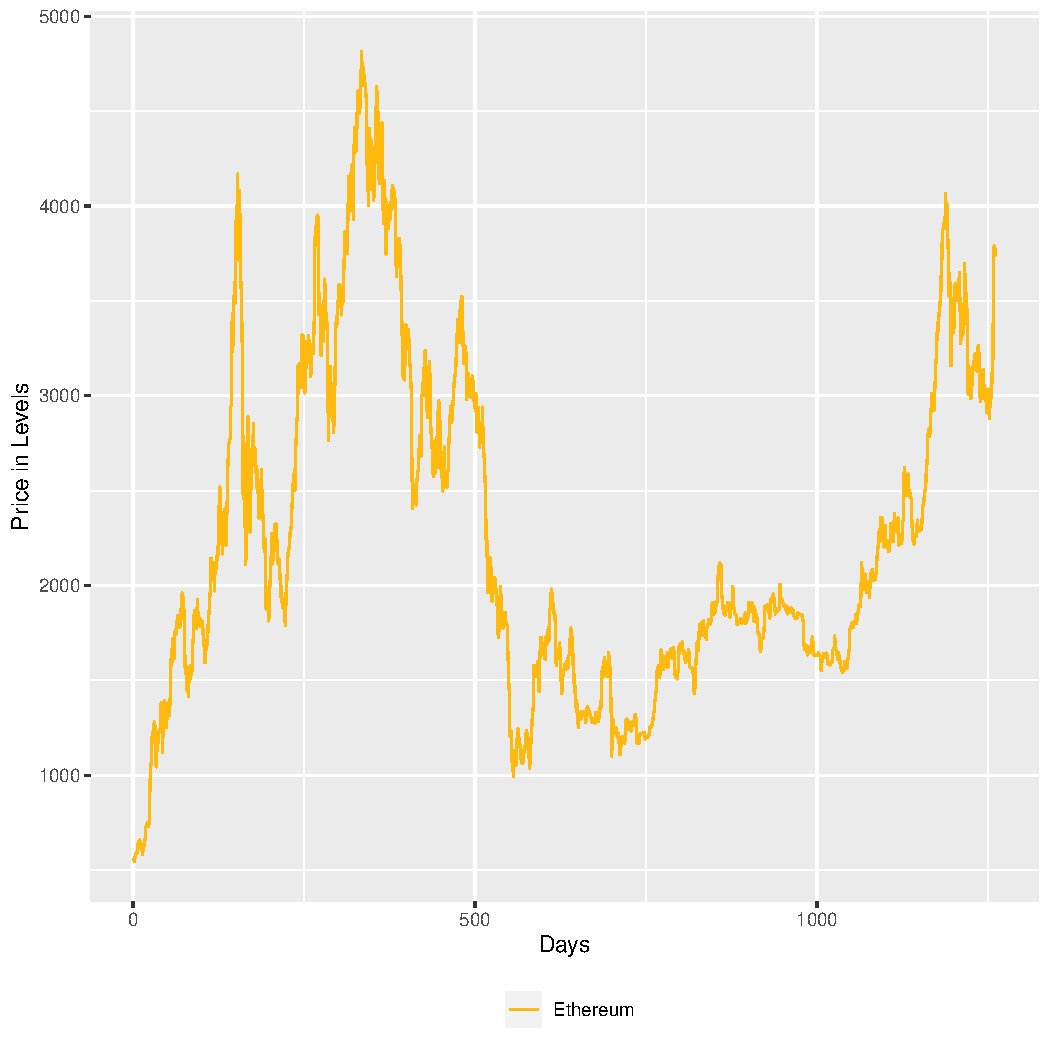
\includegraphics[width=.4\textwidth]{1.Projekt_kode/Billeder/Crypto_in_levels_Ethereum.pdf}}\\
  \subfloat[][Solana]{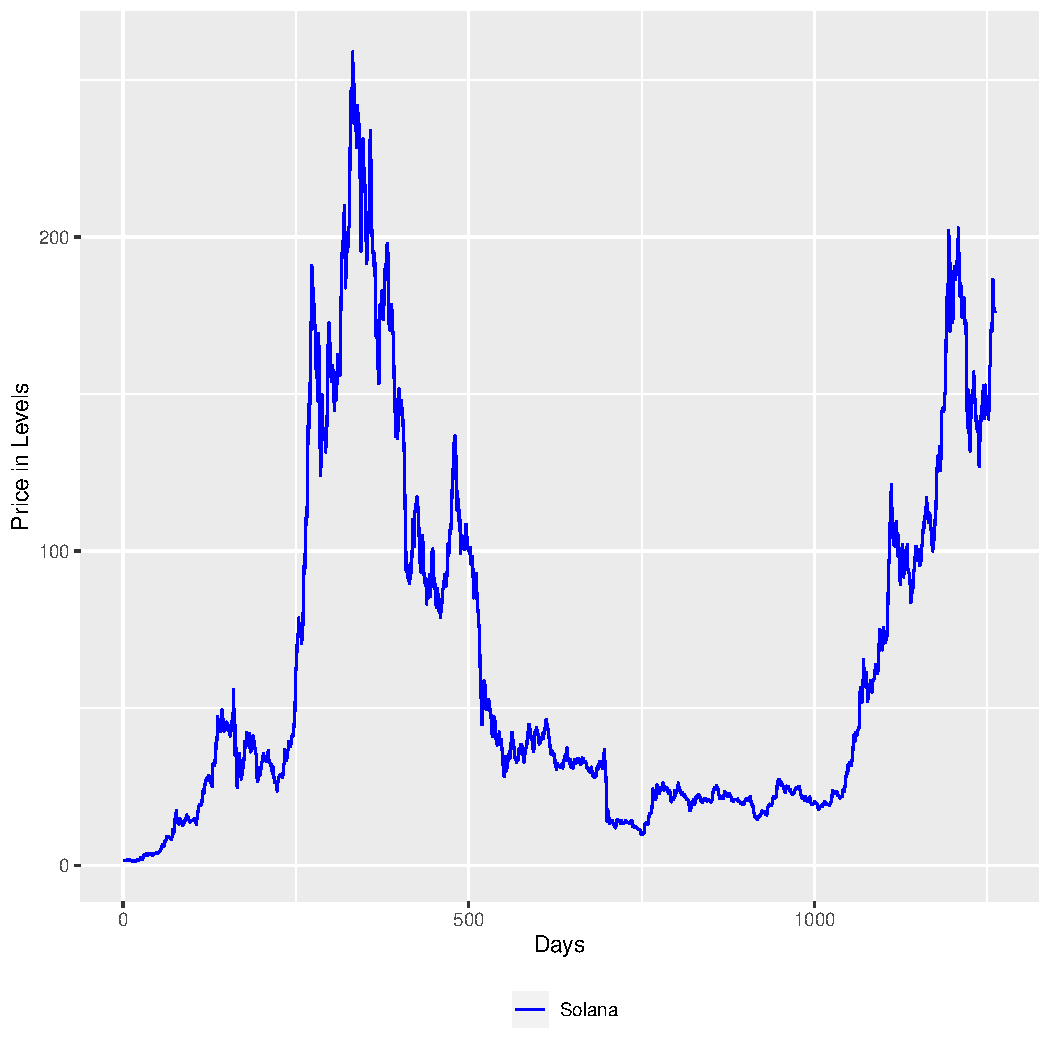
\includegraphics[width=.4\textwidth]{1.Projekt_kode/Billeder/Crypto_in_levels_Solana.pdf}}\quad
  \subfloat[][Ripple]{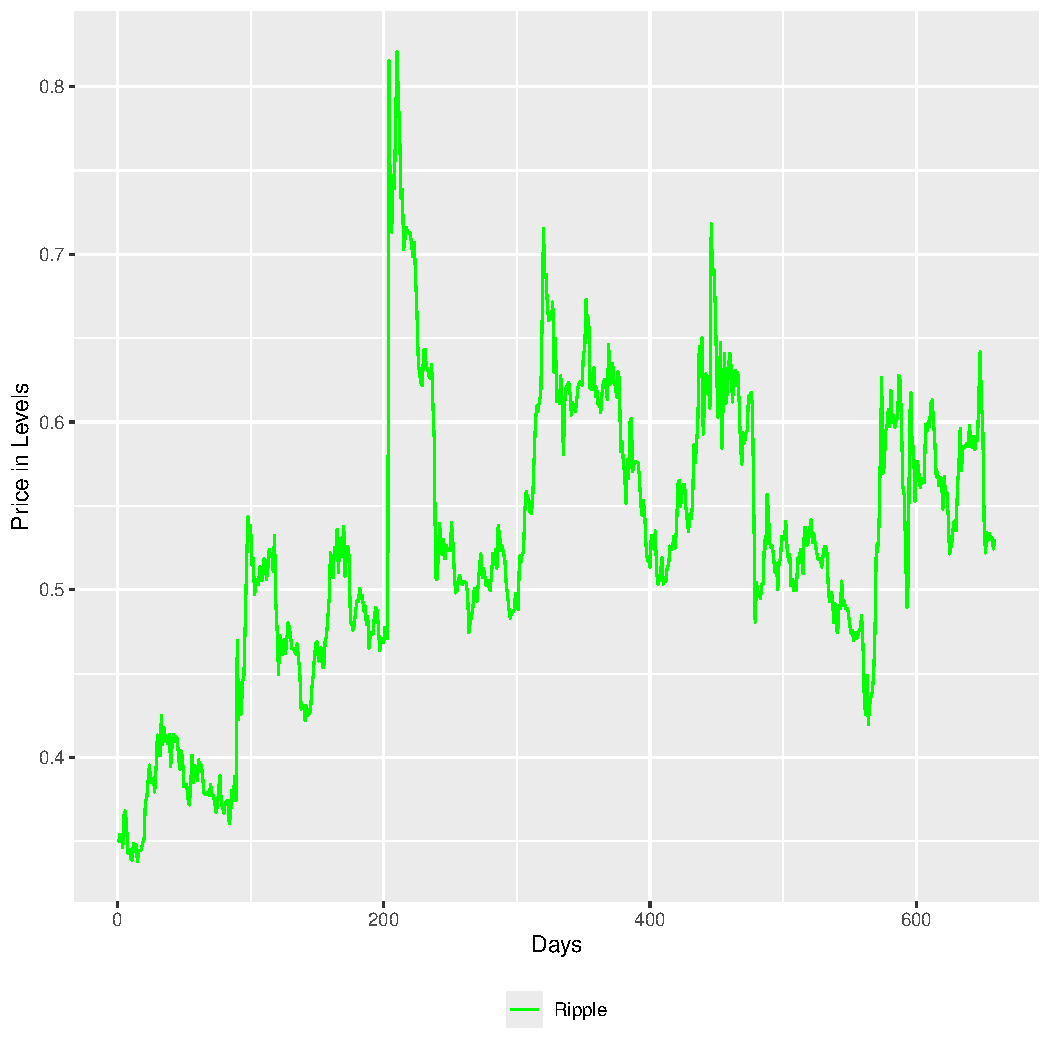
\includegraphics[width=.4\textwidth]{1.Projekt_kode/Billeder/Crypto_in_levels_Ripple.pdf}}
  \caption{Closing Prices in the Training Data}
  \label{graph_in _levels}
\end{figure}
Initially the four plots above exhibit a somewhat shared movement with a lot of similarities one of which is an explosive movement around day 1000 for BIT, ETH and SOL with these after reaching a peak all also having a steep decrease. These joint movements emphasizes the theory of having some sort of cointegrating movements. If cointegration is present then in order to forecast these prices is advantageous to incorporate 

\noindent \textbf{looking at the 4 crypto currencies there are multiple similarity's for \ref{graph_in _levels} an example of this is that a,b and c all have a rise time $1000$ and forward of our training set and all four also have a somewhat low period in the middle of the data set, other similarity's can be found but we will not go into detail about all these instead the similarity's give an occasion to look at whether cointegration is possible which can be cheeked using the Johanson, and or Engle granger. Before this can be done, other tests must be made to check whether the data even can be cointegrated this is done checking for multiple things}



Before checking for cointegration, there will be performed model validation.


\section{Model Validation}
For cointegration relations to exist, each time series must be $I(1)$. Thus each series has been differenced using the R function \textit{diff}. On this new data three graphs for each of the time series has been made. 
\begin{figure}[H]
  \centering
  \subfloat[][]{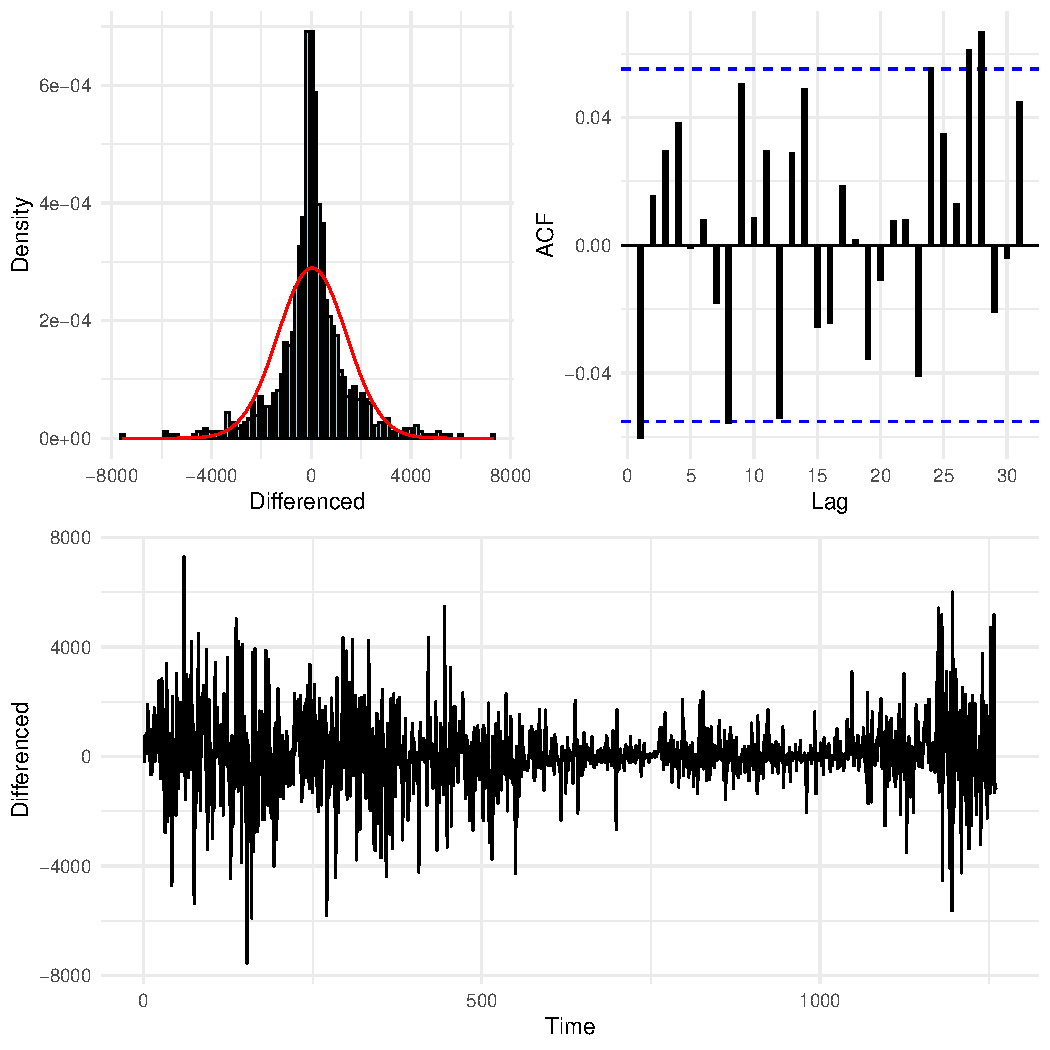
\includegraphics[width=.4\textwidth]{1.Projekt_kode/Billeder/plot_grid_Bitcoin.pdf}}\quad
  \subfloat[][]{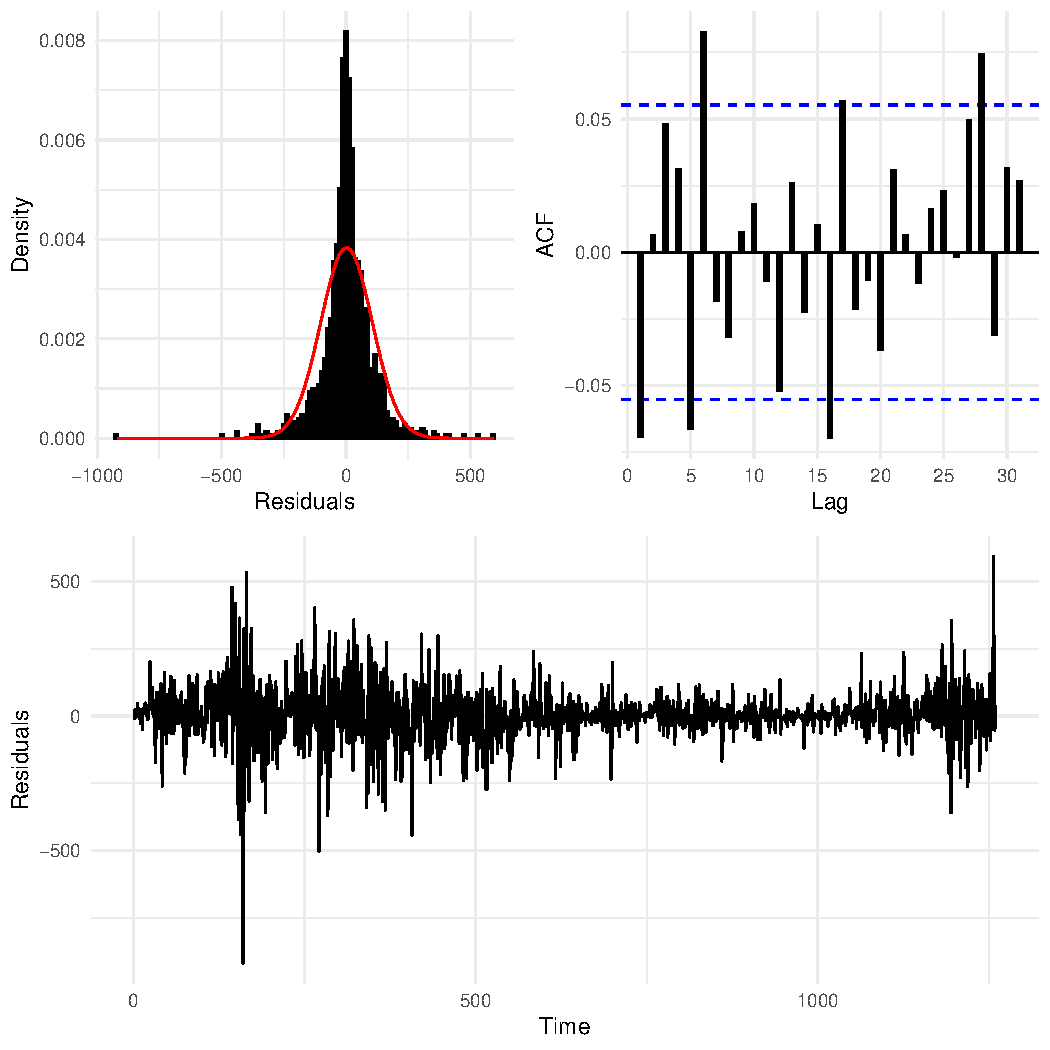
\includegraphics[width=.4\textwidth]{1.Projekt_kode/Billeder/plot_grid_Ethereum.pdf}}\\
  \subfloat[][]{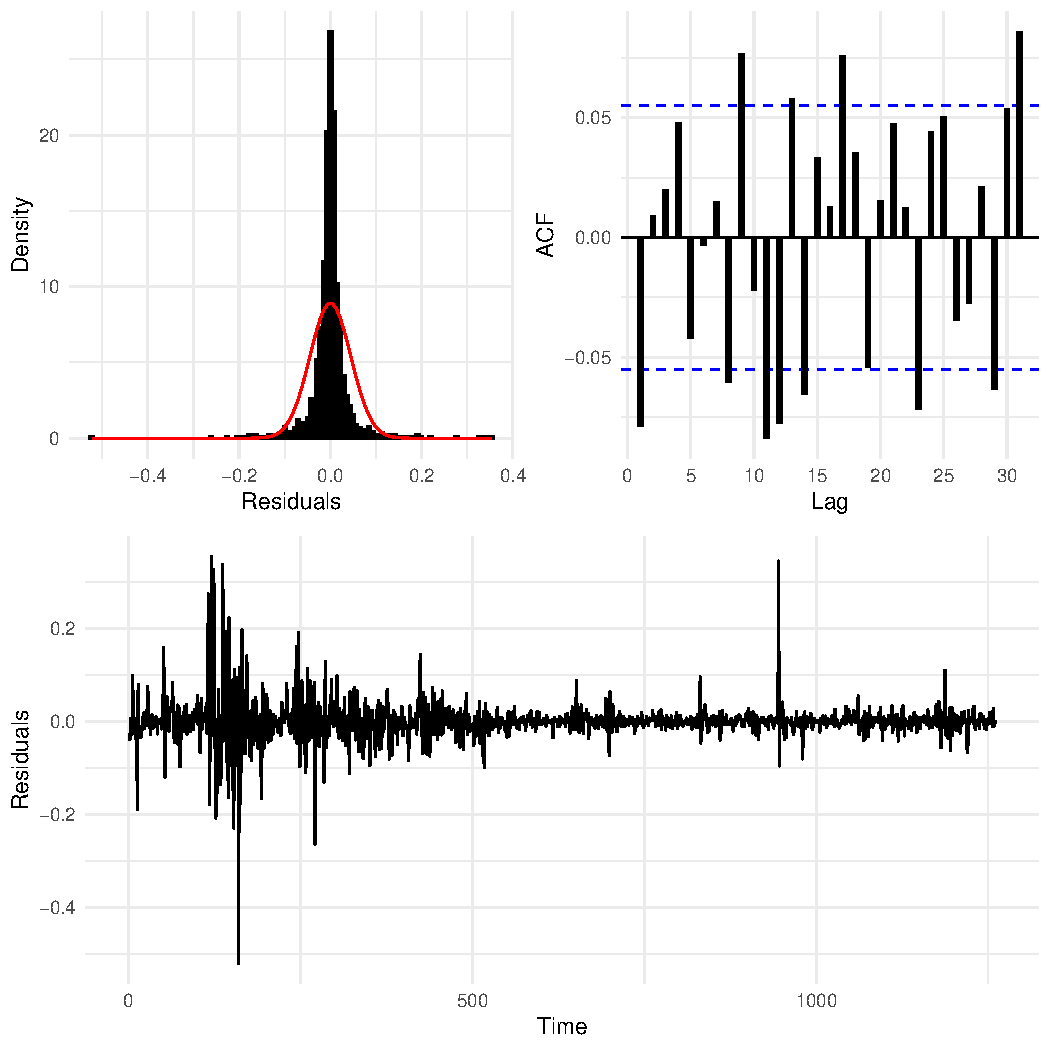
\includegraphics[width=.4\textwidth]{1.Projekt_kode/Billeder/plot_grid_Ripple.pdf}}\quad
  \subfloat[][]{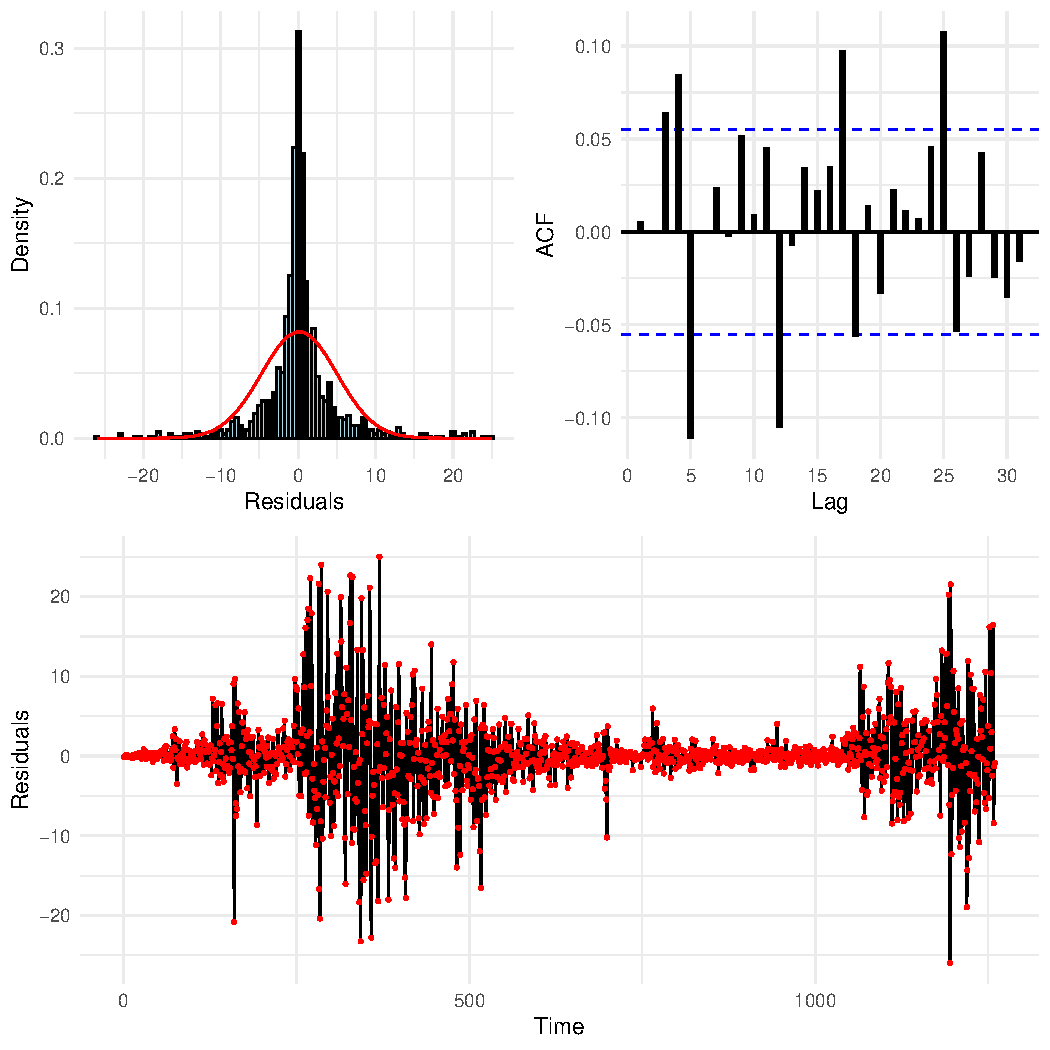
\includegraphics[width=.4\textwidth]{1.Projekt_kode/Billeder/plot_grid_Solana.pdf}}
  \caption{(a) Bitcoin, (b) Ethereum, (c) Ripple, (d) Solana }
\end{figure}
\noindent The first of the three graphs in the top left is a histogram, from which it can be inferred that the data is normally distributed with mean zero. The Second plot is an ACF plot indicating stationary data. In the last plot, the data seems to fluctuate evenly around zero, once again indicating stationary data.
Since Both the graphs and the test indicates stationary data. It can be concluded that all four time series are each individually $I(1)$.\\

\noindent Next the residuals of the optimal $VAR$ model will be examined. First the R function \textit{VARselect} will be used on the differenced data, which gives the optimal lag order based four different criteria namely AIC, HQ, BIC and FPE. Here the AIC has been chosen, and it is computed with
\begin{equation*}
    \textbf{AIC\_ligning}
\end{equation*}
The maximum lag is chosen to be $10$. The Selected lag is then $9$.\textbf{AFLÆS AIC plot, tjek den siger det samme}\\
By the use of the R function $VAR$ with the lag order specified to $9$ a $VAR(9)$ model is produced the coefficient can be found in \textbf{APPENDIX}. Next the R command \textit{checkresiduals} have been applied to the residuals of each currencies. It produce both the following plots and the Ljung-Box test. The Ljung-Box test is a statistical tool used in order to analyze if the errors exploit an uncorrelated pattern. It has the test statistic 
\begin{align*}
    Q=T(T-2)\sum^H_{h=1}\frac{r^2_{h}}{n-h}
\end{align*}
with $r$ being the accumulated sample autocorrelations, T the number of observations and H being chosen arbitrary as the maximum amount of allowed lags. This statistic is compared against the $\chi^2$ distribution and reject the null hypothesis, which is assuming the model does not exhibit a lag of fit, when
\begin{align*}
    Q>\chi^2_{1-\alpha,H}.
\end{align*}

\textbf{ANALYSE AF PLOTS}
\begin{figure}[H]
  \centering
  \subfloat[][]{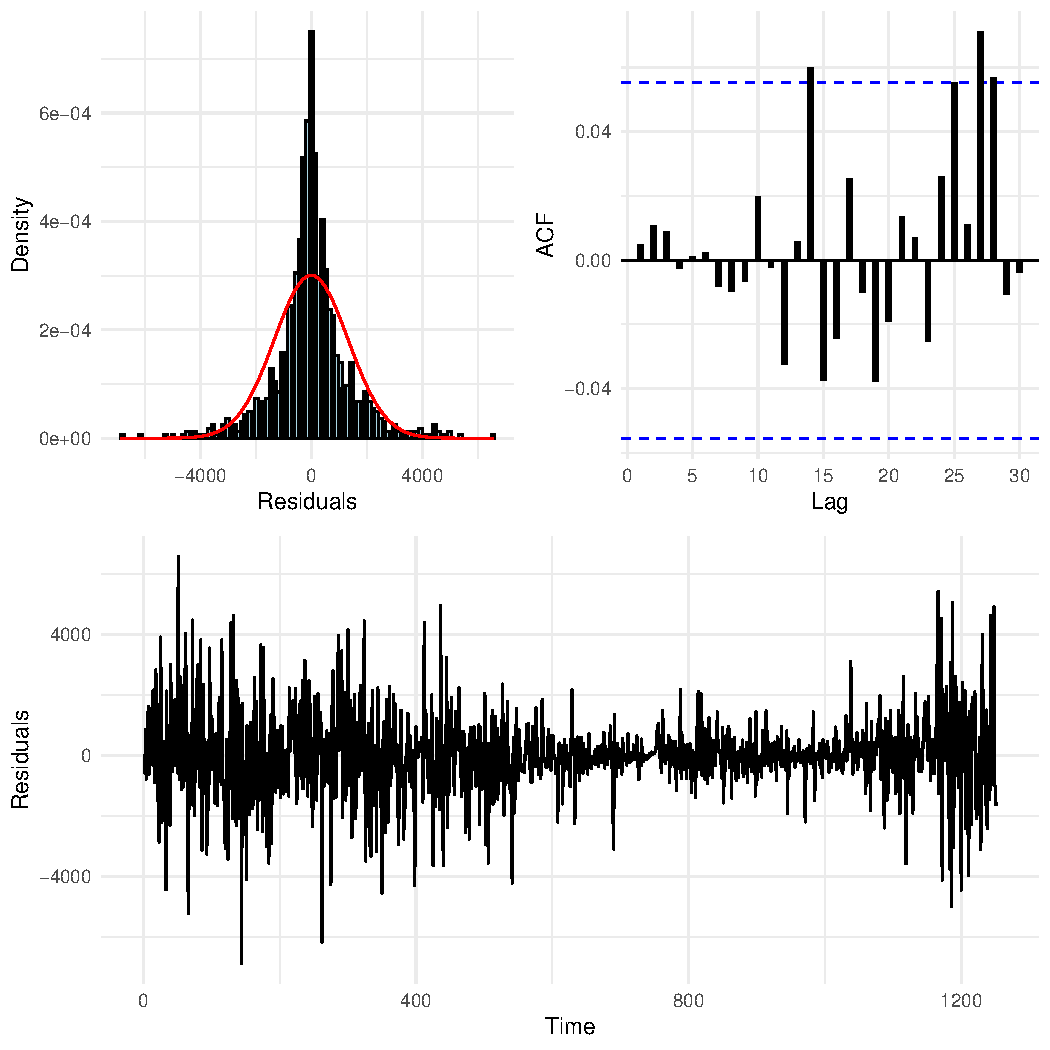
\includegraphics[width=.35\textwidth]{1.Projekt_kode/Billeder/plot_grid_ResidualsResiduals_BTC.pdf}}\quad
  \subfloat[][]{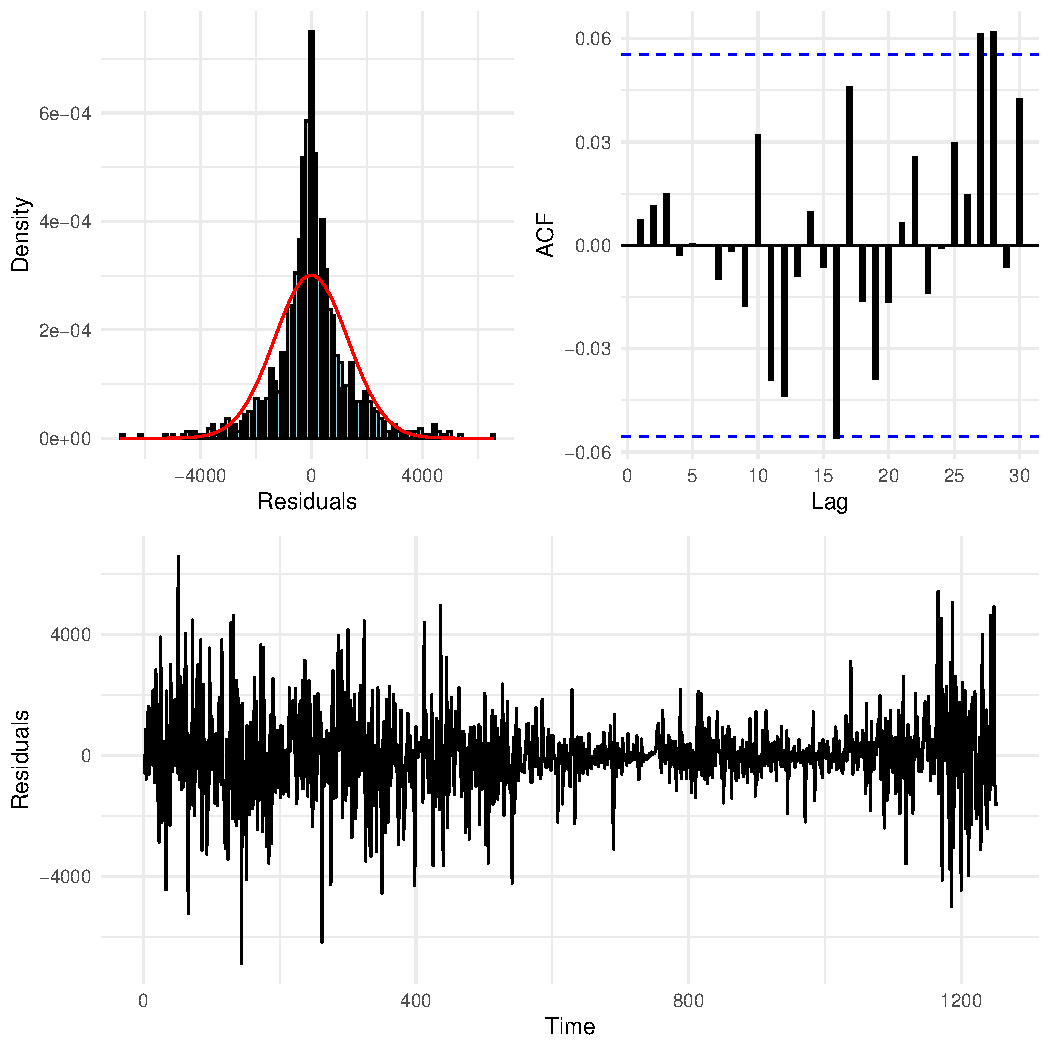
\includegraphics[width=.35\textwidth]{1.Projekt_kode/Billeder/plot_grid_ResidualsResiduals_ETH.pdf}}\\
  \subfloat[][]{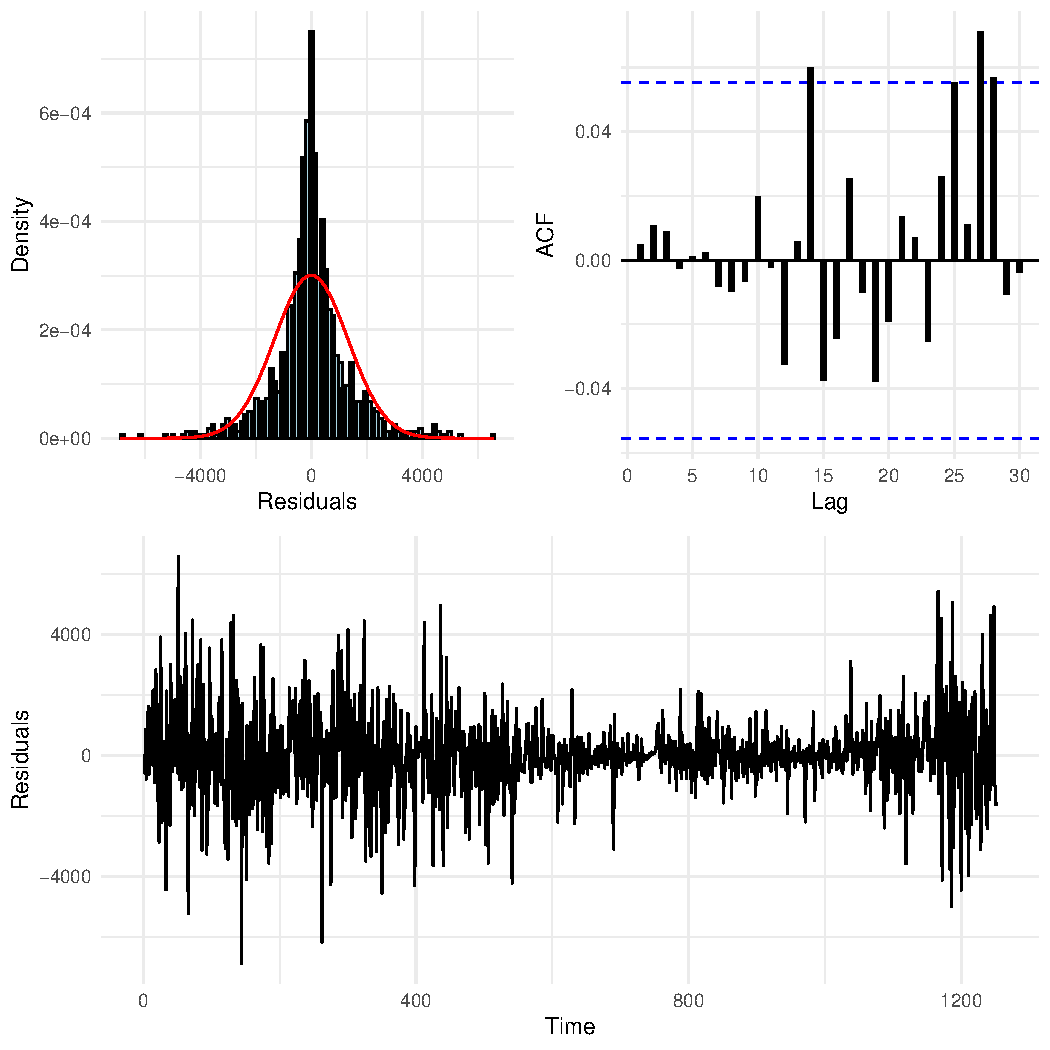
\includegraphics[width=.35\textwidth]{1.Projekt_kode/Billeder/plot_grid_ResidualsResiduals_SOL.pdf}}\quad
  \subfloat[][]{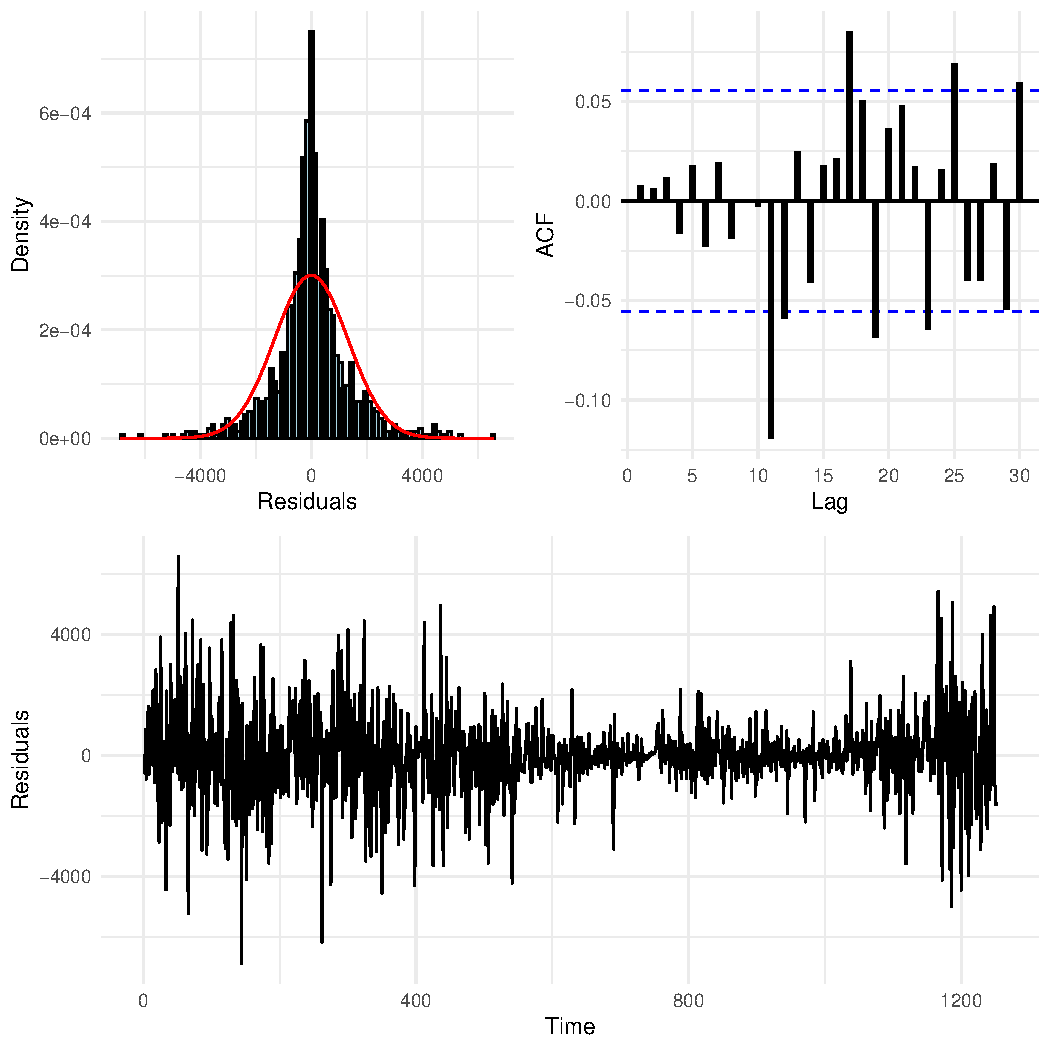
\includegraphics[width=.35\textwidth]{1.Projekt_kode/Billeder/plot_grid_ResidualsResiduals_XRP.pdf}}
  \caption{(a) Bitcoin, (b) Ethereum, (c) Ripple, (d) Solana }
\end{figure}


\textbf{Before examining whether cointegration is present it is nescessary to have the optimal amount of lags in our $VAR$ model which is done using the function $VARselect$ which provides four different tests; the AIC, HQ, BIC and FPE. Here the AIC is chosen since the AIC and BIC is preferred when forecasting. There are incentives for choosing both an AIC or BIC, the BIC is sometimes preferred for large sample sizes which is the case in this instance but in hindsight the BIC generally chooses a less complicated model since it penalizes extra parameters more than the AIC. This in unison with the fact that the BIC is often advantageous when the true model is present which we can not assume leads us to believe the AIC is more efficient since the price of cryptovalutas is also influenced by external factors not included in the model \cite{AICorBIC}.}




\newpage
\subsection{QQ-plots}

Looking at the quintile quintile plots also called QQ-plots it must be checked that the data is normally distributed and valued if there is an existence of heavy tails.
\begin{figure}[H]
  \centering
  \subfloat[][]{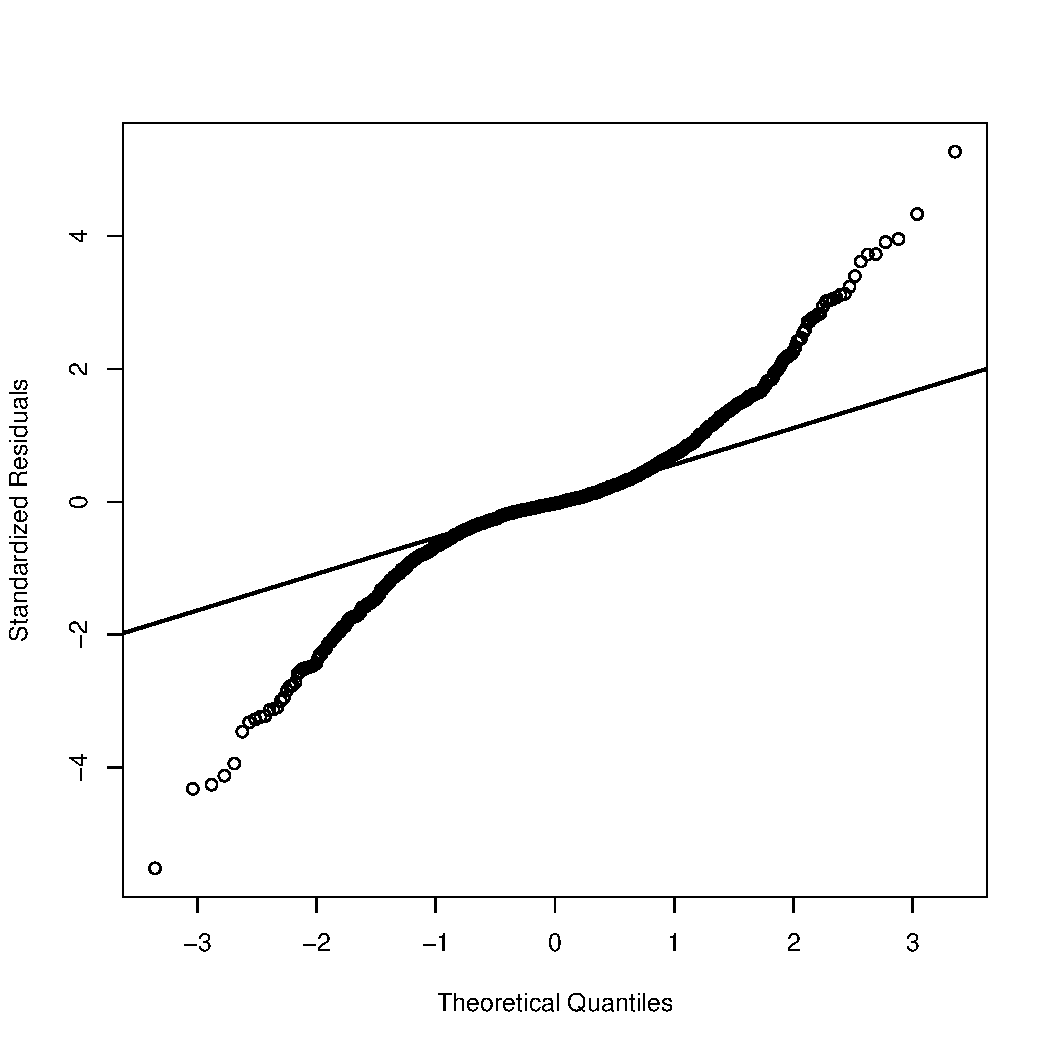
\includegraphics[width=.35\textwidth]{1.Projekt_kode/Billeder/qqplot_Bitcoin.pdf}}\quad
  \subfloat[][]{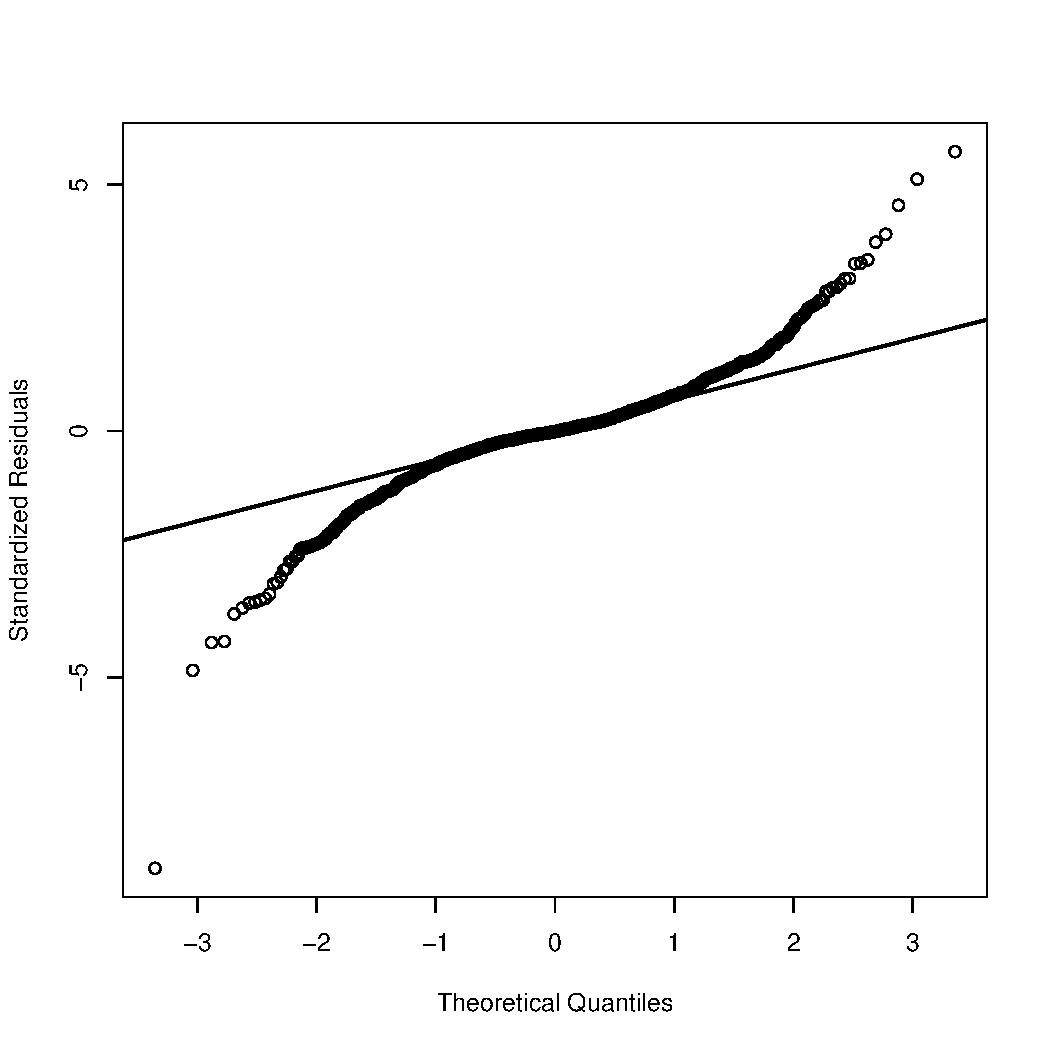
\includegraphics[width=.35\textwidth]{1.Projekt_kode/Billeder/qqplot_Ethereum.pdf}}\\
  \subfloat[][]{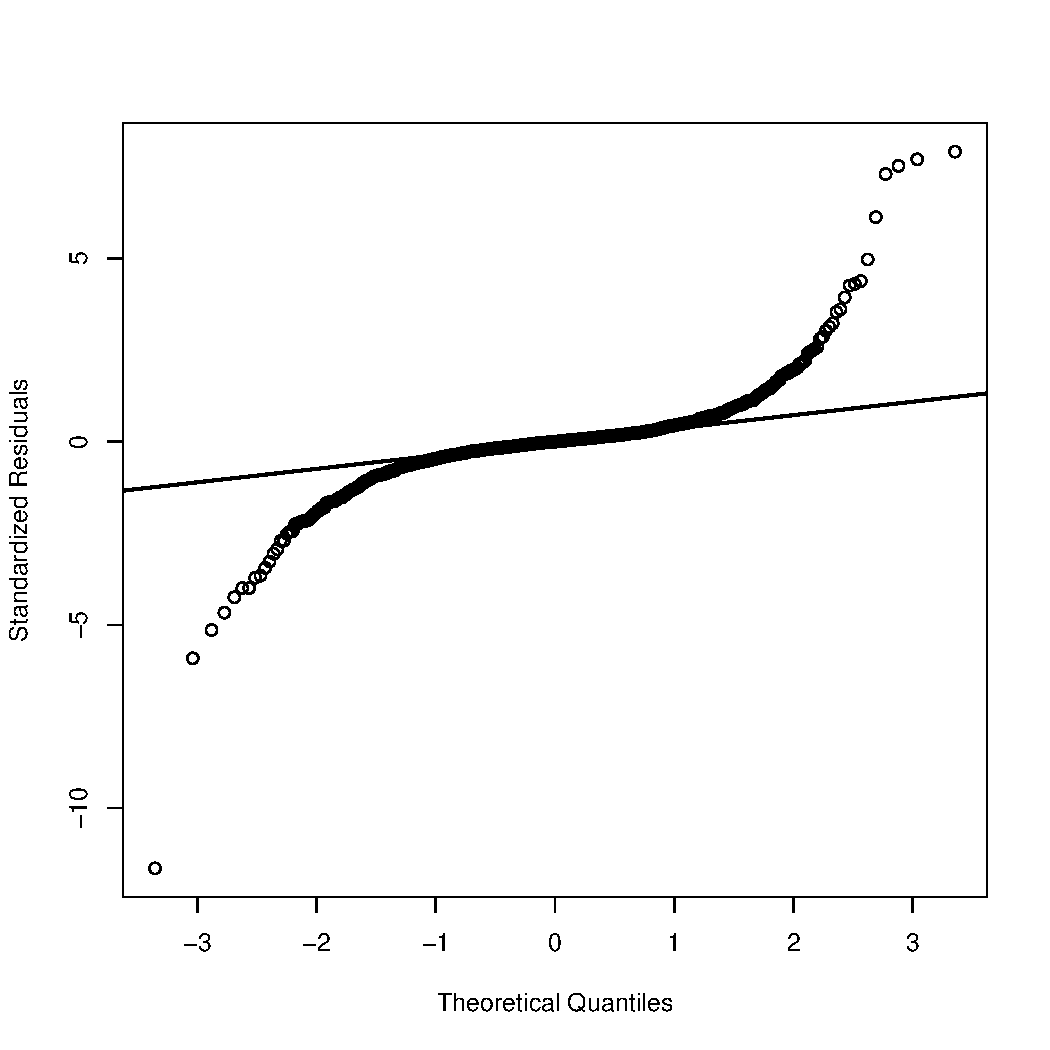
\includegraphics[width=.35\textwidth]{1.Projekt_kode/Billeder/qqplot_Ripple.pdf}}\quad
  \subfloat[][]{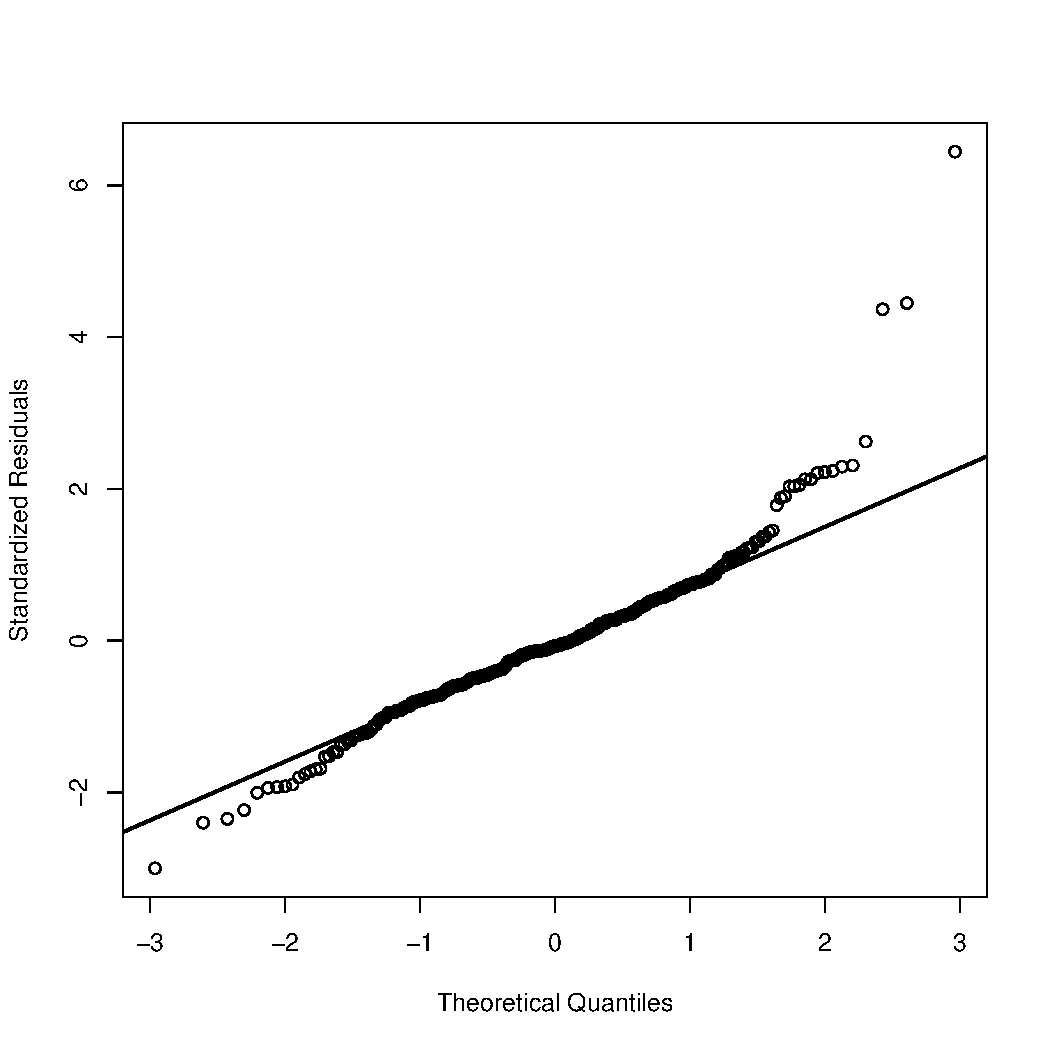
\includegraphics[width=.35\textwidth]{1.Projekt_kode/Billeder/qqplot_Solana.pdf}}
  \caption{(a) Bitcoin, (b) Ethereum, (c) Ripple, (d) Solana }
\end{figure}
Looking at the QQ-plots it clear to see that all the differenced data is symmetric in their respective QQ-plots but all have heavy tails meaning that they have more extreme values than a normal distribution, this can also be seen earlier in the histogram. This is something to consider when evaluating the model, but for now the data is still considered normally distributed.